\documentclass[a4paper, 11pt]{article}
\usepackage[table,xcdraw]{xcolor}
\usepackage{graphicx}
\usepackage{comment} % enables the use of multi-line comments (\ifx \fi) 
\usepackage{lipsum} %This package just generates Lorem Ipsum filler text. 
\usepackage{fullpage} % changes the margin

\usepackage[francais]{babel}
\usepackage[T1]{fontenc}
\usepackage[utf8]{inputenc}
\usepackage{algorithm}
\usepackage[end]{algpseudocode}

\begin{document}
%Header-Make sure you update this information!!!!
\noindent
\large\textbf{Résumé et rapport sur la sécurité} \\
\hfill Olivier Flauzac, Florent Nolot, Joffrey Hérard \\
\hfill Date: 16/06/2018 \\


\section*{Problème de départ }
Comment assurer l'identification d'un n\oe{}ud isolé (autrement appelé Device A ou Isolated Node [IN] ) tout en garantissant ses échanges avec le relais, (autrement appelé Local Gateway, LoRaGateway[LGW], Device B ). Afin qu'un ensemble d'information comme le MIC NwkSkey, AppSkey, DevEui, puisse être transporté de manière sécurisée pour pouvoir ensuite envisager un mode Proxy. 

\section*{Résumé d'un déroulement type de déploiement des capteurs.}
\paragraph{Etape 1 Initialisation :}  Aucune différence entre les devices (IN / LGW). Un premier Join Request + réception d'un Join Accept en laboratoire ( fin de conception : permet en plus un test du device) afin de récupérer les différentes informations de sessions etc.. \\
\subparagraph{Raisons}
Il est nécessaire d'avoir ces informations dès le début quelque soit le "rôle" que le device aura dans sa future localisation. Si un n\oe{}ud est isolé, ces Join Request ne seront jamais vu par Spot et, par conséquent, si un premier join n'est jamais fait, les seules informations capables d'être transmises par l'IN : \\
\begin{table}[!ht]
\centering
\caption{Données sur un IN en fonction de la réalisation de l'étape 1}
\label{Données sur un IN en fonction de la réalisation de l'étape 1}
\begin{tabular}{|l|l|l|}
\hline
Données disponible sur l'IN & Sans Join                   & Avec Join                   \\ \hline
DevEUI                     & \cellcolor[HTML]{32CB00}OUI & \cellcolor[HTML]{32CB00}OUI \\ \hline
DevNonce                   & \cellcolor[HTML]{FD6864}NON & \cellcolor[HTML]{32CB00}OUI \\ \hline
AppEUI                     & \cellcolor[HTML]{32CB00}OUI & \cellcolor[HTML]{32CB00}OUI \\ \hline
AppKey                     & \cellcolor[HTML]{32CB00}OUI & \cellcolor[HTML]{32CB00}OUI \\ \hline
AppNonce                   & \cellcolor[HTML]{FD6864}NON & \cellcolor[HTML]{32CB00}OUI \\ \hline
NwkSKey                    & \cellcolor[HTML]{FD6864}NON & \cellcolor[HTML]{32CB00}OUI \\ \hline
AppSKey                    & \cellcolor[HTML]{FD6864}NON & \cellcolor[HTML]{32CB00}OUI \\ \hline
\end{tabular}
\end{table}
\\
Si on ne fait pas un premier Join en laboratoire. L'ultime raison est celle qui permet de vérifier que le device qui essaye d'être relayé est bel est bien celui qu'il prétend être puisque il détient les éléments de sessions.
\paragraph{Etape 2  Communication en clair : } Déroulement classique comme nous l'avons entendu dès le début et que nous avons déjà programmé. Si un device une fois installé a réussi son Join Request et a eu un Join Accept. Il devient alors une LoRaGateway. Dans le cas contraire où il n'arriverait pas à être accepté. Il devient un Isolated Node. \\
L'isolated Node va voir si il peut être relayé par une LGW, il envoie donc des messages \textbf{Discover}(détaillés dans le sous paragraphe suivant). Si une LGW est à proximité de cet IN, et que la LGW est capable de gérer ce n\oe{}ud. Effectivement il reste à voir si on pose une limite du nombre de n\oe{}ud isolé géré par une LGW. Ceci n'a toujours pas été clairement définit, mais il serait plus aisé pour la LGW de faire des traitements ( en cas de chiffrement supplémentaire : à voir dans la suite de ce document). Si la LGW est capable d'accepter ce n\oe{}ud, dans ce cas celle-ci envoie un message \textbf{Accept}. Si le message est bien réceptionné  le n\oe{}ud isolé change de phase. Il passe en phase de finalisation d'enregistrement, il envoie un message \textbf{Register} avec pour cible la LGW qui lui a répondu auparavant (Par défaut c'est celle qui répond le plus vite du point de vue de l' IN). Si ce message est bien reçu alors une première demande de donnée \textbf{DataReq} est effectué de la part de la LGW à l'intention de l'IN pour finaliser l'appairage. De temps en temps (à évalué) les n\oe{}uds sont programmés pour se réveiller, pour être récoltés, ou bien pour demander aux IN attachés leurs data et renvoyer le tout en LoRaWAN.\\
\subparagraph{Contenu des messages}

\textbf{Discover} contient le type du message, l'id d'origine (Celui-ci est soit un nombre aléatoire, soit son DevEUI), la fréquence sur laquelle est émit le prochain message, pendant combien de temps le device est en phase sleep. Pendant combien de temps le device émetteur du message va écouter /et envoyer des messages. Un espace Data pour l'instant inutilisé. L'identifiant du destinataire, à ce moment là il est vide puisque le n\oe{}ud isolé ne connait pas son environnement.

\textbf{Accept} contient le type du message, l'id d'origine (Celui-ci est soit un nombre aléatoire, soit son DevEUI), la fréquence sur laquelle est émit le prochain message, pendant combien de temps le device est en phase sleep. Pendant combien de temps le device émetteur du message va écouter / et envoyer des messages. Un espace Data pour l'instant inutilisé. L'identifiant du destinataire, à ce moment là il est en fonction de l'id d'origine du message Discover.

\textbf{Register} contient le type du message, l'id d'origine (Celui-ci est soit un nombre aléatoire, soit son DevEUI), la fréquence sur laquelle est émit le prochain message, pendant combien de temps le device est en phase sleep. Pendant combien de temps le device émetteur du message va écouter / et envoyer des messages. Un espace Data pour l'instant inutilisé. L'identifiant du destinataire, à ce moment là il est en fonction de l'id d'origine du message Accept.

\textbf{DataReq} contient le type du message, l'id d'origine (Celui ci est soit un nombre aléatoire, soit son DevEUI), la fréquence sur laquelle est émit le prochain message, pendant combien de temps le device est en phase sleep. Pendant combien de temps le device émetteur du message va écouter / et envoyer des messages. Un espace Data pour l'instant inutilisé. L'identifiant du destinataire, à ce moment là il est en fonction de l'id d'origine du message Register.

\textbf{DataRes} contient le type du message, l'id d'origine (Celui-ci est soit un nombre aléatoire, soit son DevEUI), la fréquence sur laquelle est émit le prochain message, pendant combien de temps le device est en phase sleep. Pendant combien de temps le device émetteur du message va écouter / et envoyer des messages. Un espace Data. L'identifiant du destinataire, à ce moment là il est en fonction de l'id d'origine du message DataRes si celui est bien celui qui a accepté l'IN.
\newpage
\subparagraph{Schéma}
Les messages dans les schémas suivants correspondent donc à ceci : 
\begin{table}[]
\centering
\begin{tabular}{|l|l|}
\hline
ID sur schéma & Nom du message                   \\ \hline
1             & \cellcolor[HTML]{FFFFFF}Discover \\ \hline
2             & \cellcolor[HTML]{FFFFFF}Accept   \\ \hline
3             & \cellcolor[HTML]{FFFFFF}Register \\ \hline
6             & \cellcolor[HTML]{FFFFFF}DataReq  \\ \hline
7            & \cellcolor[HTML]{FFFFFF}DataRes  \\ \hline
\end{tabular}
\end{table}

\begin{figure}[!ht]    \centering
   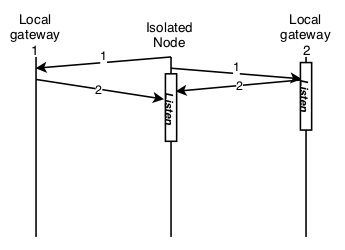
\includegraphics[scale=1]{discover.png} 
   \caption{Schéma de la phase de découverte}
   \label{Schéma de la phase de découverte}
\end{figure}

\begin{figure}[!ht]    \centering
   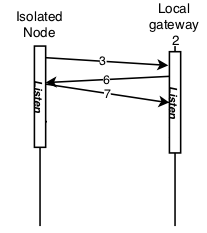
\includegraphics[scale=1]{register.png} 
   \caption{Schéma de la phase d'enregistrement}
   \label{Schéma de la phase d'enregistrement}
\end{figure}


\begin{figure}[!ht]    \centering
   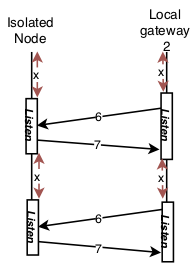
\includegraphics[scale=1]{harvest.png} 
   \caption{Schéma de la phase de récolte}
   \label{Schéma de la phase de récolte}
\end{figure}



\subparagraph{Raisons}
Ceci est notre solution décrite de bout en bout pour résoudre le problème des n\oe{}uds isolés.
\newpage
\section*{Remonté des données en LoRaWAN}

\subsection*{Concentrateur}
Classiquement, le concentrateur(LoRaGateway) récolte en LoRa toutes les données des IN, et assemble celles-ci avec sa propre data, le tout comme ceci :\\ <ID\_SOURCE1>:<DATA\_ID\_SOURCE1>:<ID\_SOURCE2>:<DATA\_ID\_SOURCE2>\\ et il remonte le tout en LoRaWAN. De notre côté on attendait une manière de décoder particulièrement le payload pour Spot.
\subsection*{Proxy}
Le relais LoRaGateway récolte en LoRa toutes les données des IN et il remonte le tout en LoRaWAN. Cette fois ci, la LoRaGateway va se faire passer pour chaque Device attaché à lui. Voici un schéma pour résumer la manière dont cela ce passera de manière globale puis comment ça se passe du point de vue de la LoRaWAN gateway 

\begin{figure}[!ht]    \centering
   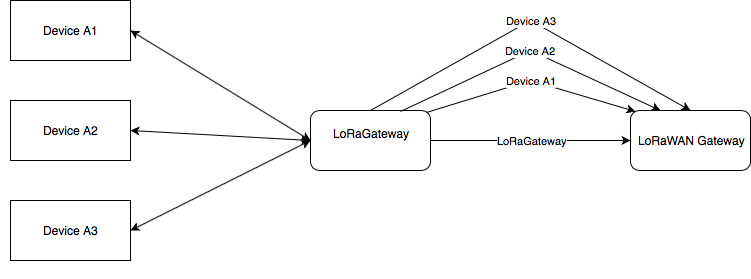
\includegraphics[scale=0.65]{diag.png} 
   \caption{Schéma d'échange d'un point de vue global}
   \label{Schéma d'échange d'un point de vue global}
\end{figure}

\begin{figure}[!ht]    \centering
   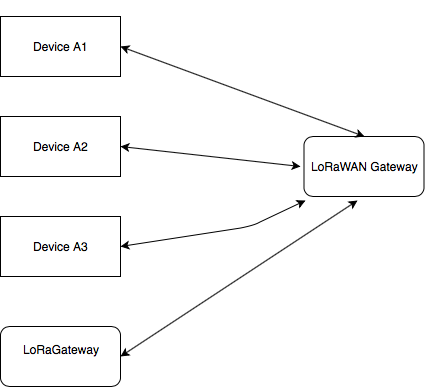
\includegraphics[scale=1]{diag2.png} 
   \caption{Schéma d'échange d'un point de vue de la gateway LoRaWAN}
   \label{Schéma d'échange d'un point de vue de la gateway LoRaWAN}
\end{figure}

\newpage
\section*{Solutions de chiffrement possibles LGW <->IN}
Afin de valider si le n\oe{}ud isolé attaché à nous est bien connu de la part de Sport. Il nous faut récupérer les informations afin de réaliser le mode proxy. C'est à dire, MIC, NwkSkey, AppSkey, DevEui, DevNonce, AppNonce, AppKey. Ces informations sont évidemment soumises à plusieurs degrés de sensibilité. Il a été convié que l'AES 128 bits, est une solution assez satisfaisante. Ce qui assure donc une sécurité de bout en bout en AES-128.

\begin{figure}[!ht]    \centering
   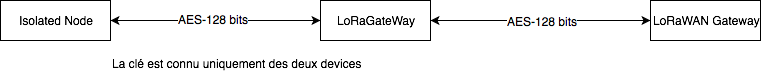
\includegraphics[scale=0.6]{aes-128.png} 
   \caption{Schéma récapitulatif sur le chiffrement}
   \label{Schéma récapitulatif sur le chiffrement}
\end{figure}
Maintenant il y a un choix important à réaliser, en effet l'AES-128 est du chiffrement symétrique. Il est nécessaire de choisir une clé qui doit être connue des deux partis (Device A et B) . \\
Nous avons donc choisi d'utiliser l'échange de clés Diffie-Hellman, qui est une méthode, publiée en 1976, par laquelle deux agents, nommés par convention Alice et Bob, peuvent se mettre d'accord sur un nombre (qu'ils peuvent utiliser comme clé pour chiffrer la conversation suivante) sans qu'un troisième agent appelé Ève puisse découvrir le nombre, même en ayant écouté tous leurs échanges. \\

Voici un déroulement de base tel que nous le concevons lors de la mise en place sur une LoRaGateway et un Isolated node.\\
La LoRaGateway choisit un nombre premier P et une base G. (P et G premier entre eux ). Dans notre exemple, P=23 et G=3\\
la LoRaGateway choisit un nombre secret a=6\\
Elle envoie à Bob la valeur A = $g^a$ [mod P] = $3^6$ [23] = 16\\
Bob choisit à son tour un nombre secret b=15\\
Bob envoie à la LoRaGateway la valeur B = $G^b$ [mod P] = 3\up{15} [23] = 12\\
la LoRaGateway peut maintenant calculer la clé secrète : $B^a$ [mod P] = $12^6$ [23] = 9\\
Bob fait de même et obtient la même clé que la LoRaGateway : $A^b$ [mod P] = 16\up{15} [23] = 9\\

Pour faire simple, La LoRaGateway peut transmettre toutes les données nécessaire en clair c'est à dire P, G, A  à un n\oe{}ud isolé et cela sans aucun soucis. Puisque pour déduire la clé résultante il faut résoudre l'impossibilité (calculatoire) de déduire des seules informations $g^a$, $g^b$, G et P, la valeur de G\up{ab} .
il faut toutefois parler du problème de l'attaque classique du Man in the middle. La parade classique à cette attaque consiste à signer les échanges de valeurs à l'aide d'une paire de clés asymétriques certifiées par une tierce partie fiable, ou dont les moitiés publiques ont été échangées auparavant par les deux participants.

\section*{Problème final }
Lors d'un test rapide, la plupart des services qui utilisent l'algorithme de Diffie-Hellman, est gérée par la bibliothèque libre OpenSSL. La force de cet algorithme réside aussi dans les principes mathématiques qu'entourent les nombres premiers, tout comme pour l'algorithme RSA, plus le nombre premier choisi est grand plus la sécurité en est renforcée. Or plus un nombre est grand.. plus il faut s'attendre à gérer des opérations mathématiques très lourdes, en plus de la recherche initiale du nombre premier. Ce qui rappelons le, peut être assez long compte tenu de la puissance de calcul dont dispose un capteur. Ceci n'est que le problème au niveau de la recherche de P. En effet on parle d'une élévation à la puissance (dans la suite du calcul) d'un nombre déjà extrêmement grand, en effet il faut s'attendre à exploser la capacité maximale que peut engranger un nombre en informatique c'est à dire : 18 446 744 073 709 551 615 == 2\up{64}-1 . Pour résoudre ce souci OpenSSL utilise la bibliothèque BIGNUM en C . Qui comme la lib OpenSSL n'est pas disponible sur les capteurs sur lesquels nous développons. 
\section*{Conclusion}
Il y a plusieurs piste à envisager, celle dont-on parle dans ce document part du principe que nous n'avons aucune autre entrée sécurisée donnée par la LoRaWAN Gateway lors d'un join. La solution à ce problème est probablement du côté des fonctions de type courbes elliptiques comme celles de Diffie-Hellmann . Pour faire simple une solution basée sur les courbes elliptiques serait non implémentable \textbf{sans secure element} . Il est donc nécessaire d'envisager une autre piste. 


\end{document}